\documentclass[xcolor=dvipsnames]{beamer}

% ==== 主題 ====
\usetheme{CambridgeUS}
\usefonttheme{professionalfonts}          % 不覆蓋你自訂的字型

% ==== 字型 ====
\usepackage{fontspec}
\usepackage{xeCJK}
\renewcommand{\familydefault}{\rmdefault} % 使用 serif 字體(重點)

% 西文字型:Times New Roman 的開源替代品
\setmainfont{TeX Gyre Termes}[
  Ligatures=TeX,
  BoldFont={* Bold},
  ItalicFont={* Italic}
]

% 中文字型(可改為思源宋體、標楷體等)
\setCJKmainfont{Noto Serif CJK TC}
\setCJKsansfont{Noto Sans CJK TC} % 有需要再用
\setCJKmonofont{Noto Sans Mono CJK TC}

% ==== 數學字型(與正文字體一致)====
\usepackage{unicode-math}
\setmathfont{TeX Gyre Termes Math}

% ==== 套件 ====
\usepackage{amsmath, amssymb}
\usepackage{graphicx}
\usepackage{hyperref}
\usepackage{minted}
\usepackage{fvextra}
\usepackage{xcolor}
\usepackage{tikz}
\usetikzlibrary{arrows.meta}


% ==== 顏色設定(可選)====
\definecolor{MyBlue}{RGB}{3, 55, 105}
\setbeamercolor{structure}{fg=MyBlue}
\setbeamercolor{block title}{bg=MyBlue,fg=white}
\setbeamercolor{block body}{bg=blue!5}

\setminted{
    linenos,                % 行號
    frame=lines,            % 上下框線
    framesep=5pt,           % 程式碼與邊框距離
    numbersep=8pt,          % 行號與程式碼距離
    fontsize=\scriptsize,   % 字體大小
    breaklines,             % 自動換行
    tabsize=4,              % tab 寬度
    rulecolor=\color{black},% 框線顏色
    xleftmargin=1.5em       % 左側縮排
}

% % 去掉 Section N,但保留原有樣式(顏色/字型/間距)
% \makeatletter
% \defbeamertemplate{section page}{nonumber}{
%   \begingroup
%     \centering
%     \vfill
%     % 大多數 theme 的 section page 都用這個顏色盒與字型;因此能保留原樣式
%     \begin{beamercolorbox}[sep=12pt,center]{section title}
%       \usebeamerfont{section title}\insertsectionhead\par
%     \end{beamercolorbox}
%     \vfill
%   \endgroup
% }
% \makeatother

% % 啟用我們的無編號樣式
% \setbeamertemplate{section page}[nonumber]

% % 若有自動插入章節頁
% \AtBeginSection{\frame[plain]{\sectionpage}}



\sloppy
\setlength{\emergencystretch}{2em}  % 加大緊急伸縮
\title{肺部電腦斷層掃描之非小細胞癌 PD-L1 表現預測:}
\subtitle{結合多任務自監督學習與生成對抗網路}
\author{TAI, WEI HSUAN}

\date{August 2025}

\begin{document}
	
	\begin{frame}
		\titlepage
	\end{frame}
    
    % 大綱
	\begin{frame}
		\frametitle{Outline}
        \begin{itemize}
            \item 研究動機
            \item 研究背景
            \item 模型介紹
            \item 研究方法
            \item 結果與討論
            \item 結論與展望
        \end{itemize}
	\end{frame}

    \section{研究動機}
    \begin{frame}
        \sectionpage
    \end{frame}
    % 研究動機
    \begin{frame}
        \frametitle{研究動機}
        \begin{itemize}
            \item 癌症是全球主要的死亡原因之一,肺癌是其中最
            \item 肺癌是台灣癌症死亡率最高的癌症類型。
            \item 台灣每年有超過 1 萬人死於肺癌
        \end{itemize}
    \end{frame}

    % 113台灣癌症統計資料
    \begin{frame}
        \frametitle{研究動機}
        \begin{figure}
            \centering
            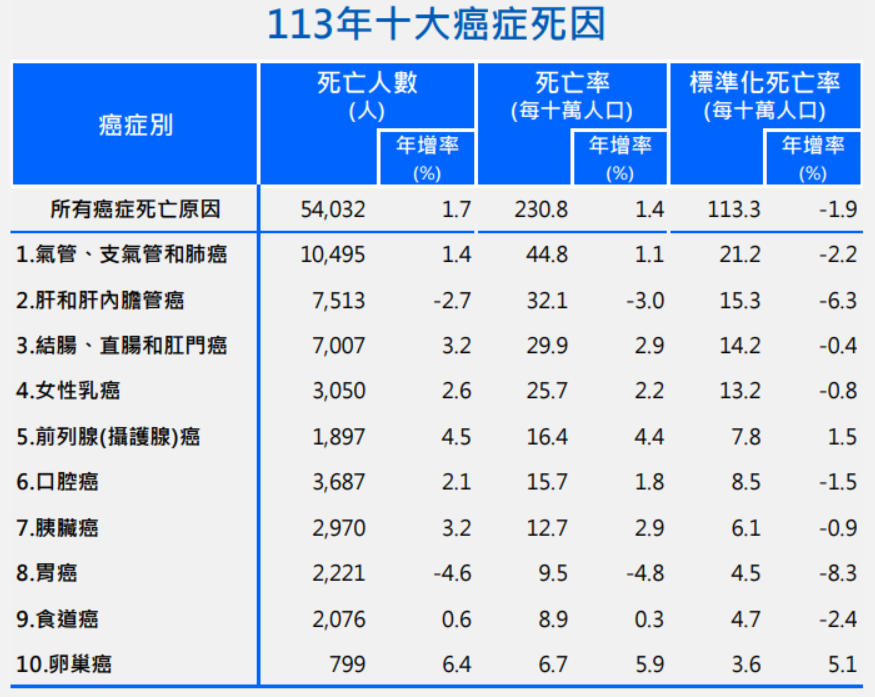
\includegraphics[width=0.6\textwidth]{src/TW_113cancer_stat.png}
            \caption{113 年台灣癌症統計資料}
            \label{fig:113tw_cancer_stat}
        \end{figure}
    \end{frame}

    \section{研究背景}
    \begin{frame}
        \sectionpage
    \end{frame}
    % 研究背景
    \begin{frame}
        \frametitle{研究背景}
        \begin{itemize}
            \item 癌症的早期診斷和預後評估對於提高治療效果至關重要。
            \item 免疫檢查點抑制劑(Immune checkpoint inhibitors, ICIs)已成為治療肺癌的重要手段。
            \item PD-L1 表達水平是評估 ICIs 治療效果的關鍵生物標誌物。
            \item 傳統的 PD-L1 評估方法依賴於組織切片,存在侵入性和時間延       
        \end{itemize}
    \end{frame}


    % 癌症的分類
    \begin{frame}
        \frametitle{癌症的分類}
        \begin{itemize}
            \item 非小細胞肺癌(Non-small-cell lung carcinoma, NSCLC):
                \begin{itemize}
                    \item 佔肺癌的約85 \%。
                    \item 包括腺癌、鱗狀細胞癌和大細胞癌等類型。
                    \item 生長較慢,預後較好。
                \end{itemize}

            \item 小細胞肺癌(Small-cell lung carcinoma, SCLC):
                \begin{itemize}
                    \item 佔肺癌的約15 \%。
                    \item 通常與吸煙有關。
                    \item 生長迅速,易於轉移。
                \end{itemize}

        \end{itemize}
    \end{frame}

    \section{模型介紹}
    \begin{frame}
        \sectionpage
    \end{frame}

    % 模型介紹
    \begin{frame}
        \frametitle{模型介紹}
        本專題使用或參考了以下的幾個模型及架構:
        \begin{itemize}
            \item Mask Image Model (MIM)
            \item Masked Autoencoder (MAE)
            \item Vision Transformer (ViT)
            \item Multi-task Masked Autoencoder (MT-MAE)
            \item Simple Contrastive Learning (SimCLR)
            \item Global Contrastive Masked Autoencoder (GCMAE)
            \item Contrastive Masked Autoencoder (CMAE)
        \end{itemize}
    \end{frame}

    % Mask Image Model (MIM)
    \begin{frame}
        \frametitle{Masked Image Model (MIM)}
        \begin{itemize}
            \item 分成 pretrain, finetune
            \item 利用Transfer Learning的概念,將 pretrain 的 encoder 應用於下游任務
            \item pretrain 階段,將輸入影像隨機遮蔽一部分,並預測被遮蔽的部分以學習特徵
        \end{itemize}
    \end{frame}

    % Masked Autoencoder (MAE)
    \begin{frame}
        \frametitle{Masked Autoencoder (MAE)}
        \begin{itemize}
            \item MIM 的一種變體
            \item 利用 Autoencoder 補全被遮蔽的部分以學習特徵
            \item 將 pretrain 的 encoder 應用於下游任務(如:應用於 ViT 模型以進行分類任務)
        \end{itemize}
    \end{frame}

    % MAE architecture
    \begin{frame}
        \begin{figure}
            \centering
            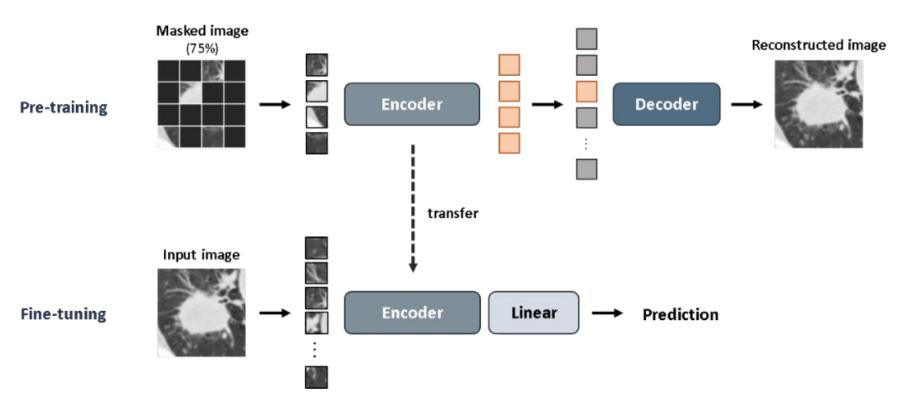
\includegraphics[width=1\textwidth]{src/MAE.png}
            \caption{Masked Autoencoder (MAE) 的架構}
            \label{fig:mae_architecture}
        \end{figure}
        圖片來源:周姵妤學姐的碩士論文
    \end{frame}

    % Vision Transformer (ViT)
    \begin{frame}
        \frametitle{Vision Transformer (ViT)}
        \begin{itemize}
            \item 將影像分割成 patches,並將其視為序列輸入到 Transformer 模型中
            \item 利用自注意力機制學習影像特徵
            \item 使用 CLS token 或是 GAP 處理 token 之後丟到 linear layer 進行分類
        \end{itemize}
    \end{frame}

    % Vision Transformer (ViT) architecture
    \begin{frame}
        \begin{figure}
            \centering
            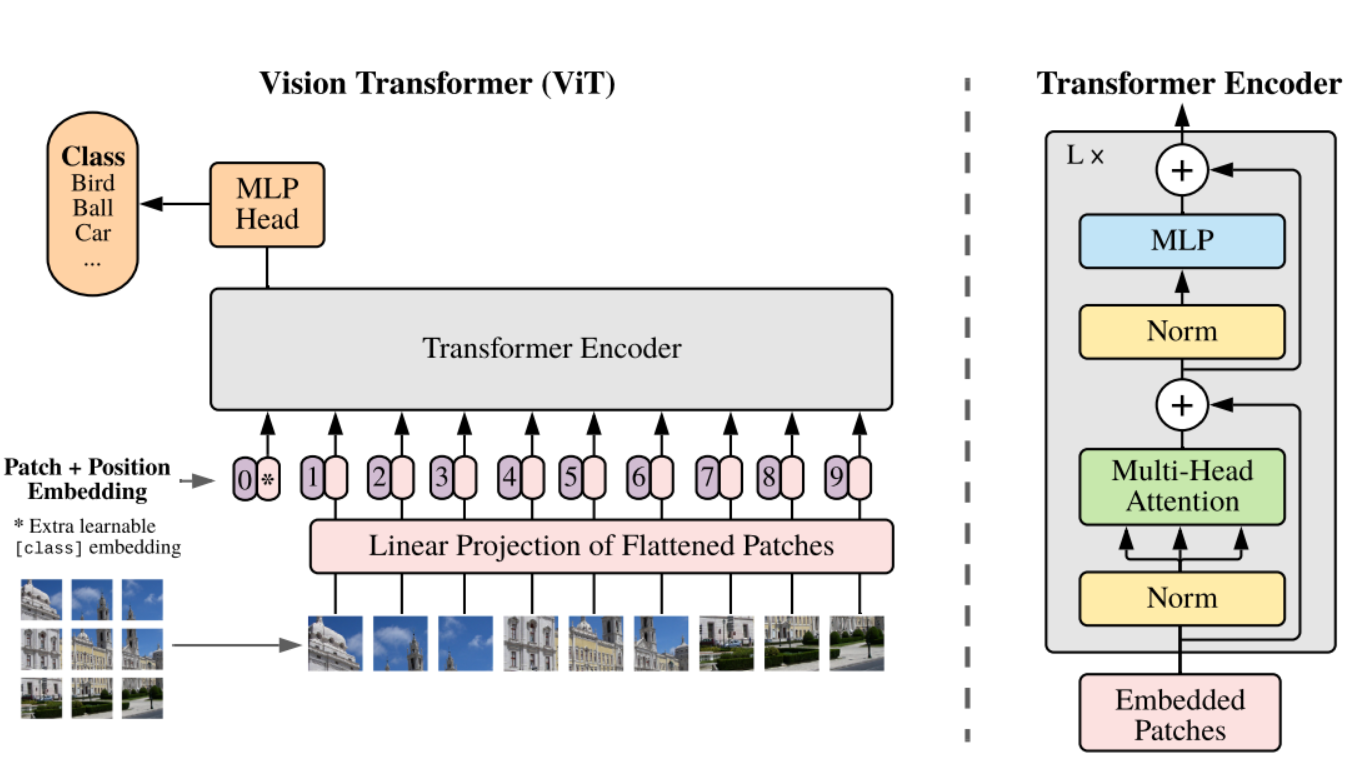
\includegraphics[width=0.8\textwidth]{src/ViT.png}
            \caption{Vision Transformer (ViT) 的架構}
            \label{fig:vit_architecture}
        \end{figure}
        圖片來源:\url{https://arxiv.org/abs/2010.11929}
    \end{frame}

    % Multi-task Masked Autoencoder (MT-MAE)
    \begin{frame}
        \frametitle{Multi-task Masked Autoencoder (MT-MAE)}
        \begin{itemize}
            \item 使用大量 GAN 生成的影像進行 pretrain
            \item 在 pretrain 階段將 MAE 與分割任務結合,使用混合的 Loss 進行優化
            \item 使用訓練好的 encoder 作為下游分割任務的 backbone
        \end{itemize}
    \end{frame}

    % MT-MAE architecture
    \begin{frame}
        \begin{figure}
            \centering
            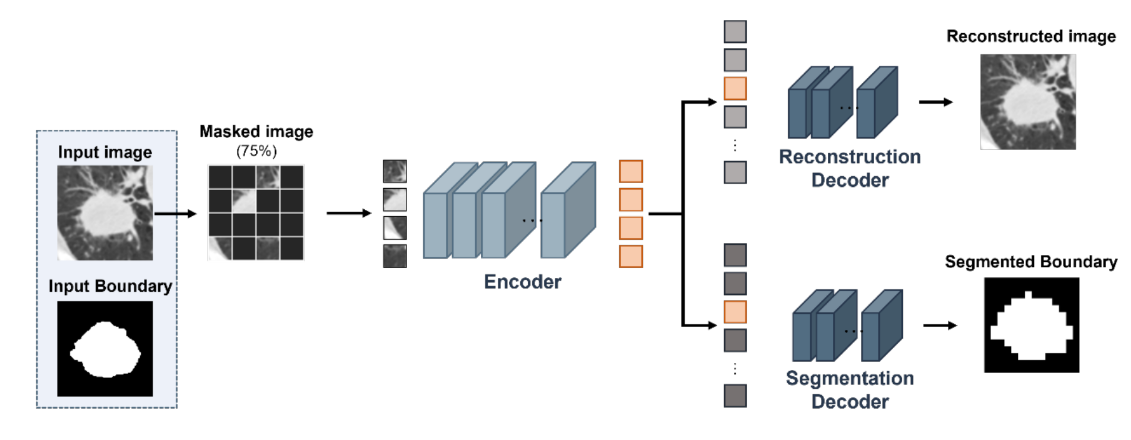
\includegraphics[width=1\textwidth]{src/MTMAE.png}
            \caption{Multi-task Masked Autoencoder (MT-MAE) 的架構}
            \label{fig:mtmae_architecture}
        \end{figure}
        圖片來源:周姵妤學姐的碩士論文
    \end{frame}

    % Simple Contrastive Learning (SimCLR)
    \begin{frame}
        \frametitle{Simple Contrastive Learning (SimCLR)}
        \begin{itemize}
            \item 透過對比學習學習影像特徵
            \item 對同一張影像進行不同的增強,並將其視為正樣本;將不同的影像視為負樣本,使模型學習拉近正樣本,遠離負樣本
            \item 使用 NT-Xent loss 進行優化
        $$
        \ell_{i,j} = -\log \frac{\exp(\mathrm{sim}(\mathbf{z}_i, \mathbf{z}_j)/\tau)}{
            \sum_{k=1}^{2N} \mathbb{1}_{k \neq i}\exp(\mathrm{sim}(\mathbf{z}_i, \mathbf{z}_k)/\tau)}
        $$
        \end{itemize}
    \end{frame}
    % SimCLR architecture
    \begin{frame}
        \begin{figure}
            \centering
            \begin{tikzpicture}
                \node at (0,1.8) (h) {$\longleftarrow\,$Representation$\,\longrightarrow$};
                \node[draw, circle] at (0,-1) (x) {$\,~\mathbf{x}~\,$};
                \node[draw, circle] at (-2.5,0) (x1) {$\tilde{\mathbf{x}}_i$};
                \node[draw, circle] at (2.5,0) (x2) {$\tilde{\mathbf{x}}_j$};
                \node at (-2.5,1.8) (h) {$\mathbf{h}_i$};
                \node at (2.5,1.8) (c) {$\mathbf{h}_j$};
                \node at (-2.5,3) (hh) {$\mathbf{z}_i$};
                \node at (2.5,3) (cc) {$\mathbf{z}_j$};
                \path[->] 
                    (x)  edge [>=latex] node[below,rotate=-25] {$t\sim\mathcal{T}$} (x1)
                    (x)  edge [>=latex] node[below,rotate=25] {$t'\sim \mathcal{T}$} (x2)
                    (x1)  edge [>=latex] node[left,rotate=0] {$f(\cdot)$} (h)
                    (x2)  edge [>=latex] node[right,rotate=0] {$f(\cdot)$} (c)
                    (h)  edge [>=latex] node[left,rotate=0] {$g(\cdot)$} (hh)
                    (c)  edge [>=latex] node[right,rotate=0] {$g(\cdot)$} (cc);
                \path[<->]
                    (hh)  edge [>=latex] node[above,rotate=0] {Maximize agreement} (cc);
            \end{tikzpicture}
            \caption{SimCLR 架構圖}
        \end{figure}
    \end{frame}

    % Global Contrastive Masked Autoencoder (GCMAE)
    \begin{frame}
        \frametitle{Global Contrastive Masked Autoencoder (GCMAE)}
        \begin{itemize}
            \item 結合 MAE 與 SimCLR 的思想
            \item 利用 MAE 學習局部特徵;結合 GCLR 學習全局特徵
        \end{itemize}
    \end{frame}

    % GCMAE architecture
    \begin{frame}
        \begin{figure}
            \centering
            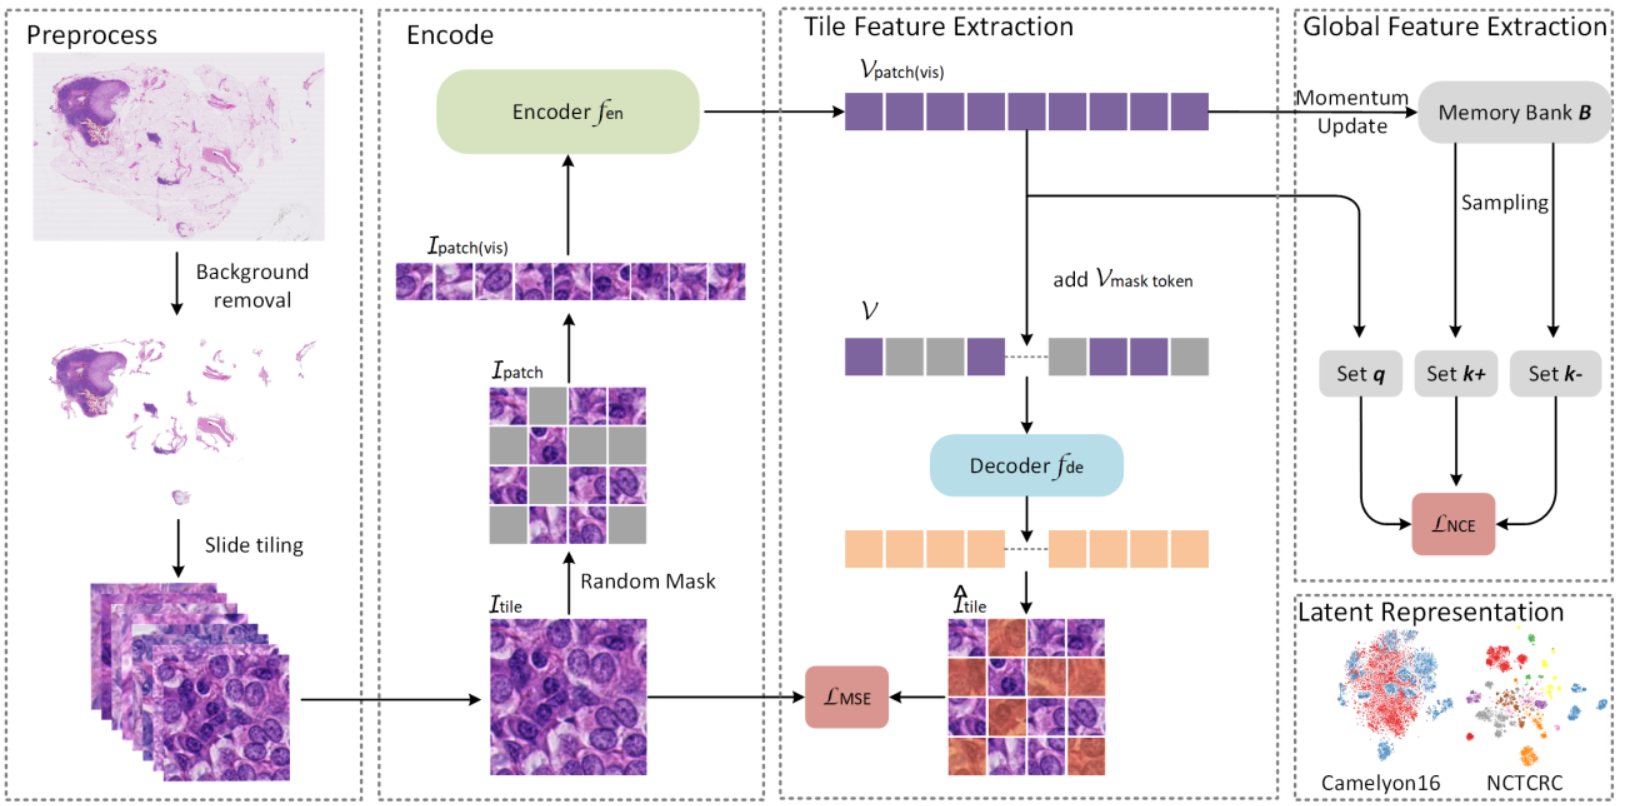
\includegraphics[width=1\textwidth]{src/GCMAE.png}
            \caption{Global Contrastive Masked Autoencoder (GCMAE) 的架構}
            \label{fig:gcmae_architecture}
        \end{figure}
        圖片來源:\url{https://arxiv.org/abs/2205.09048}
    \end{frame}

    % Contrastive Masked Autoencoder (CMAE)
    \begin{frame}
        \frametitle{Contrastive Masked Autoencoder (CMAE)}
        \begin{itemize}
            \item 一樣結合 MAE 與對比學習
            \item 利用孿生網路結構,將 MAE 的 encoder 與對比學習的 encoder 結合
        \end{itemize}
    \end{frame}

    % CMAE architecture
    \begin{frame}
        \begin{figure}
            \centering
            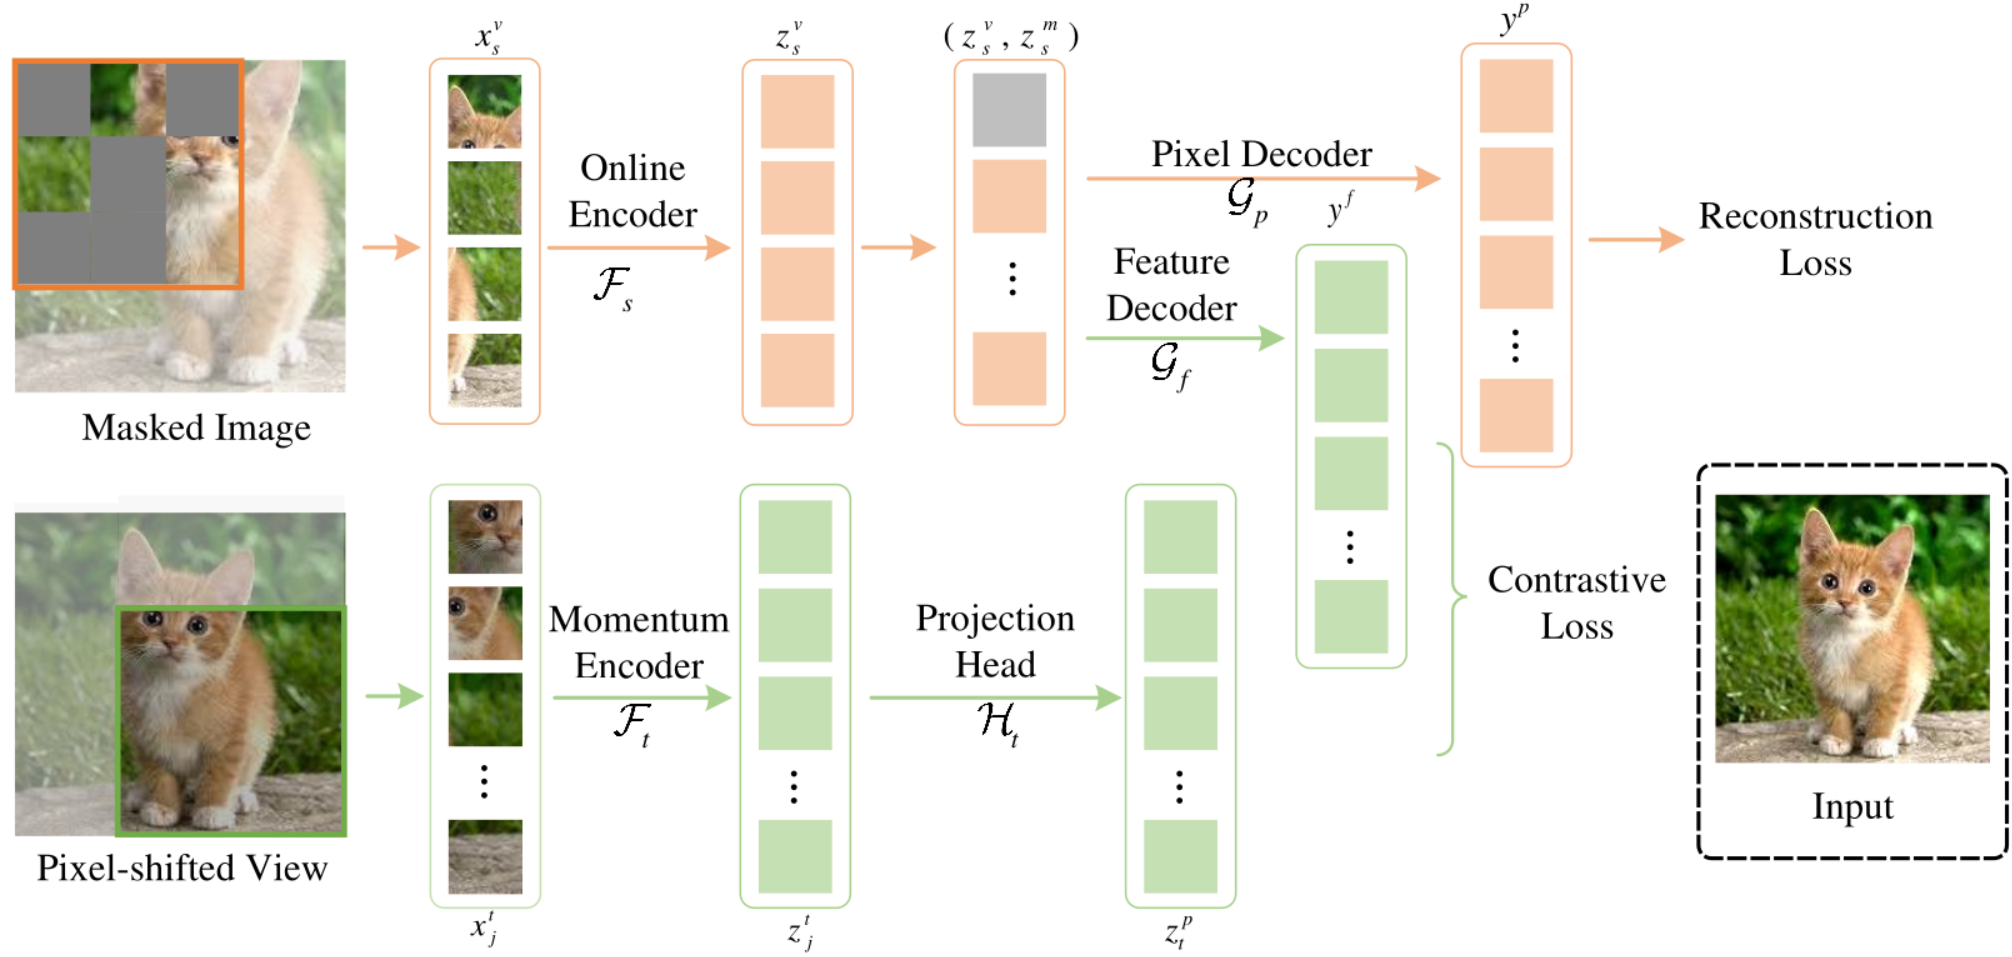
\includegraphics[width=1\textwidth]{src/CMAE.png}
            \caption{Contrastive Masked Autoencoder (CMAE) 的架構}
            \label{fig:cmae_architecture}
        \end{figure}
        圖片來源:\url{https://arxiv.org/abs/2207.13532}
    \end{frame}

    \section{研究方法}
    \begin{frame}
        \sectionpage
    \end{frame}

    % 研究方法
    \begin{frame}
        \frametitle{預訓練階段}
        \begin{enumerate}
            \item 使用 SimCLR 繼續訓練 MTMAE 的 encoder
            \item 純粹使用 SimCLR 訓練 encoder
            \item 將 encoder 替換成 CMAE 的 encoder
        \end{enumerate}
    \end{frame}

    \begin{frame}
        \frametitle{微調的方法}
        \begin{figure}
            \centering
            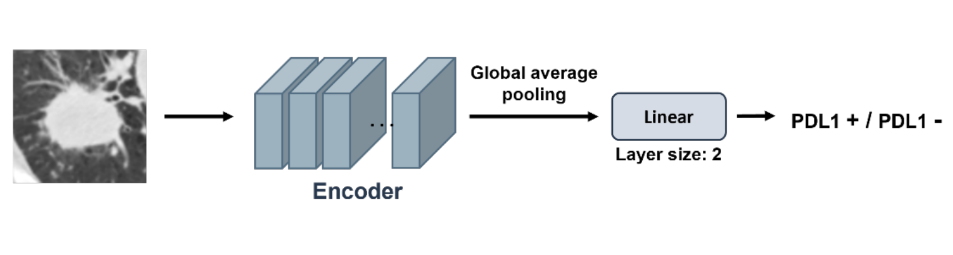
\includegraphics[width=0.8\textwidth]{src/finetune.png}
            \caption{微調階段的架構}
            \label{fig:finetune_architecture}
        \end{figure}
    \end{frame}

    \begin{frame}
        \frametitle{Reference}
        \begin{itemize}
            \item \url{https://github.com/tianyicui/pack/blob/master/V2.pdf}
            \item \url{https://oi-wiki.org/dp/}
            \item \url{https://atcoder.jp/contests/dp/tasks}
            \item \url{https://leetcode.com/problem-list/dynamic-programming/}
            
            
        \end{itemize}
    \end{frame}
\end{document}